\documentclass[tikz,border=5mm]{standalone}
\usepackage{tikz}
\usetikzlibrary{arrows.meta}
\usepackage{amsmath}
\usepackage{physics}

\ExplSyntaxOn
\msg_redirect_name:nnn { siunitx } { physics-pkg } { none }
\ExplSyntaxOff

\begin{document}
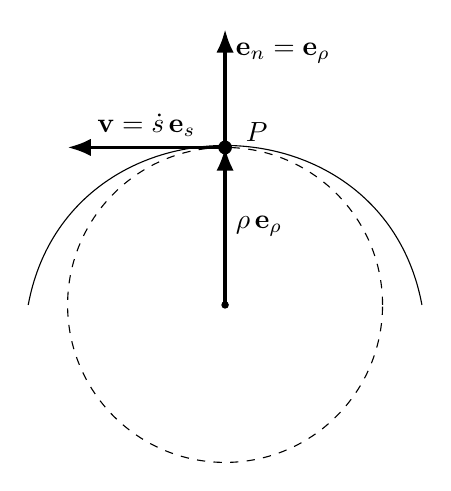
\begin{tikzpicture}[scale=2,
		vector/.style={-{Latex}, very thick}]

    \node at (0.2, 1.1) {$P$};

	\draw [dashed] (0, 0) circle (1);
	\draw [fill] (0, 0) circle (0.02);
	\draw [fill] (0, 1) circle (0.04);

    \draw [vector] (0, 0) -- (0, 1) node [midway, right] {$\rho \, \vb{e}_{\rho}$};
    \draw [vector] (0, 1) -- (-1, 1) node [midway, above] {$\vb{v} = \dot{s} \, \vb{e}_{s}$};
    \draw [vector] (0, 1) -- (0, 1.75) node [pos=0.8, right] {$\vb{e}_{n} = \vb{e}_{\rho}$};

    \draw (-1.25, 0) .. controls (-1, 1.35) and (1, 1.35) .. (1.25, 0);

\end{tikzpicture}
\end{document}